\documentclass[11pt,a4paper]{article}
\usepackage[margin=2.5cm]{geometry}
\usepackage{amsmath,amssymb}
\usepackage{booktabs}
\usepackage{graphicx}
\usepackage{caption}   % \captionof, for the non-floating tables
\usepackage[hidelinks]{hyperref}

% Figure paths are relative to the repository root; build from there.
\graphicspath{{./}{../}}

% Let floats fill a page rather than deferring a whole block to the next one.
\renewcommand{\topfraction}{0.9}
\renewcommand{\bottomfraction}{0.8}
\renewcommand{\textfraction}{0.07}
\renewcommand{\floatpagefraction}{0.75}

\title{American Option Pricing with Alternatives to Deep Neural Networks\\
       \large Results Summary}
\author{}
\date{\today}

\begin{document}
\maketitle

\noindent This is an interim summary: 1 of 4 planned approximation methods is complete, and a cross-method comparison follows once more than one is finished.

The task is to predict the price of an American option from six inputs: asset price, maturity, rate, dividend, implied volatility, and the price of the corresponding European option. The dataset is proprietary and is not distributed with the code.

\section{One-Dimensional Generalized Stochastic Sampling (gSS)}

Following Antonov and Piterbarg (2021), gSS approximates the target as a linear
combination of $N$ product kernels centred on stochastically sampled nodes
$z_n \in \mathbb{R}^D$ (their eqs.~25 and~30):
%
\begin{align}
  \tilde{f}(x) &= \sum_{n=1}^{N} \beta_n
      \prod_{d=1}^{D} \psi\!\big( (x_d - z_{n,d})\,\omega_d \big),
      \label{eq:gss-model} \\[2pt]
  \omega_d &= \theta\,\kappa_d,
      \qquad \kappa_d = \bar{g}_d / \Delta z,
      \label{eq:freq-bounds} \\[2pt]
  \beta(\theta) &= \arg\min_{\beta}
      \big\lVert \Psi(\theta)^{\top}\beta - Y \big\rVert_2^{2}
      + \lambda \lVert \beta \rVert_2^{2}.
      \label{eq:ridge}
\end{align}
%
Here $\psi$ is the inverse quadratic kernel, $\Delta z$ the mean nearest-node
distance, and $\bar{g}_d$ the relative directional risk magnitudes estimated from
the gradients of a base fit. Only the coefficients $\beta$ are regressed; the
nodes are fixed and the single scalar $\theta$ is chosen by a bounded
one-dimensional search. Ridge rather than plain least squares is required because
the Gram matrix is near-degenerate at this node count.

The node count is then enriched from $N$ to $N'$ for evaluation, and $\theta$
re-calibrated on the dense set, because the optimum moves with node density: the
value fitted on the sparse set is not the one to use at test time.

Fitted on 70\,318 rows and evaluated on a held-out test set of 30\,137 rows, 6 features.

On held-out data the enriched model reaches a relative $L_2$ error of 0.0032, against 0.0027 in sample. Both figures come from the same $N'$-node model, so the gap between them measures generalisation directly. It is small, and shows no sign of overfitting.

\paragraph{Interpretation.} No baseline has been computed yet. The European
option price is one of the six inputs and is itself a strong predictor of the
American price, so some share of this accuracy comes from that input rather than
from the method. Baselines follow with the cross-method comparison.

\begin{center}
\begin{minipage}{\linewidth}\centering
  \begin{minipage}[t]{0.48\linewidth}\vspace{0pt}\centering
    \begin{tabular}{lr}
      \toprule
      Simulation range & 4 \\
      Nodes (fit model) & 1\,000 \\
      Nodes (test model) & 5\,000 \\
      Kernel & \texttt{invquad} \\
      Node placement & \texttt{random} \\
      Kernel scale $\theta$ & 2 \\
      Ridge $\lambda$ & $1\times10^{-6}$ \\
      Floating-point precision & \texttt{float64} \\
      Random seed & 1 \\
      \bottomrule
    \end{tabular}
  \end{minipage}\hfill
  \begin{minipage}[t]{0.48\linewidth}\vspace{0pt}\centering
    \begin{tabular}{lr}
      \toprule
      Test $L_2$ (dense) & 0.0032 \\
      Train $L_2$ (dense) & 0.0027 \\
      Test MAE (dense) & 0.0017 \\
      Train MAE (dense) & 0.0016 \\
      Train $L_2$ (fit model) & 0.0053 \\
      Train MAE (fit model) & 0.0031 \\
      \bottomrule
    \end{tabular}
  \end{minipage}
  \captionof{table}{Configuration (left) and accuracy (right).}
  \label{tab:onedim_gss}
\end{minipage}
\end{center}

\begin{figure}[htbp]
  \centering
  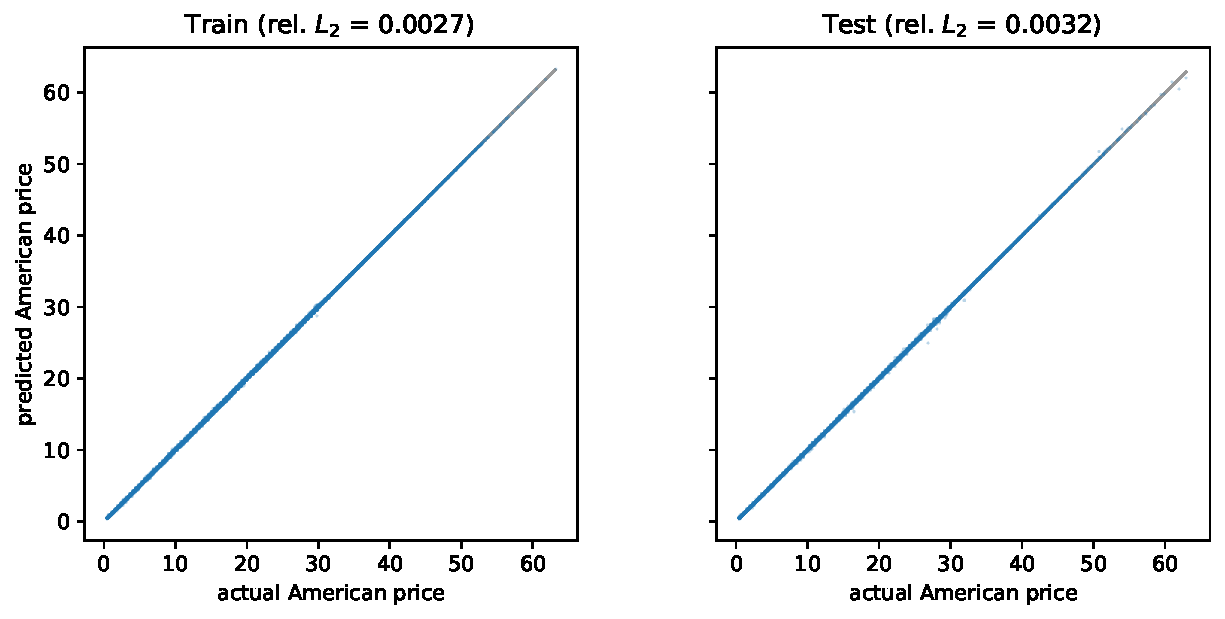
\includegraphics[width=\linewidth]{figures/onedim-gss-fit.pdf}
  \caption{Predicted against actual American option price, with the $y = x$ reference in grey.}
  \label{fig:onedim-gss-fit}
\end{figure}

\begin{figure}[htbp]
  \centering
  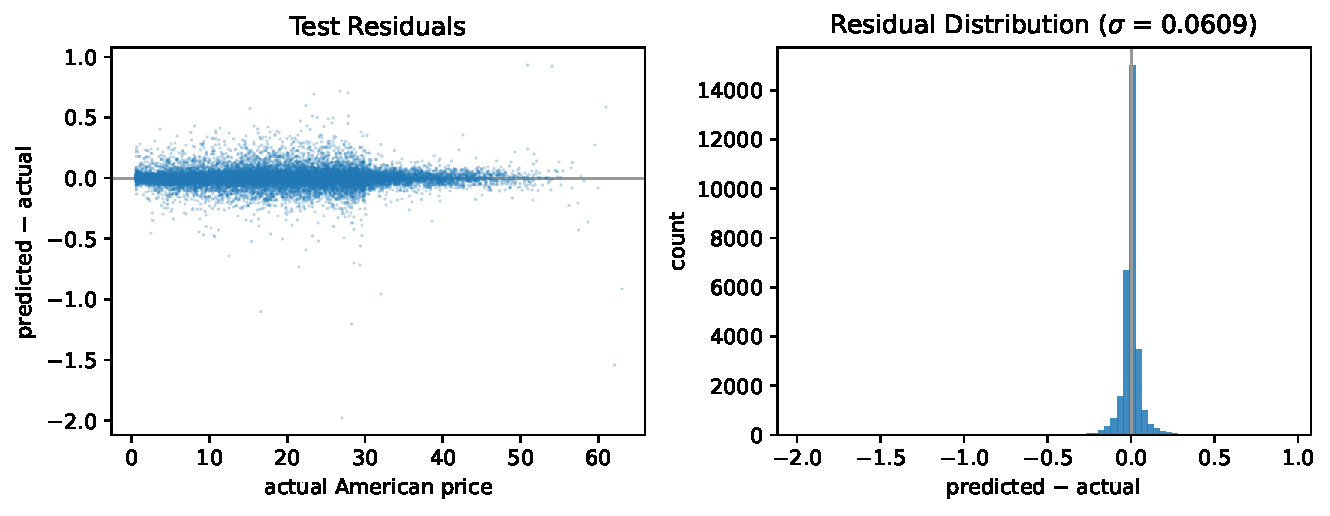
\includegraphics[width=\linewidth]{figures/onedim-gss-residuals.pdf}
  \caption{Test residuals against actual price, and their distribution.}
  \label{fig:onedim-gss-residuals}
\end{figure}

\end{document}
